An alternative to finite differences that avoids rounding errors is based on complex variable analysis. 
The first proposals originated in 1967 using the Cauchy integral theorem involving the numerical evaluation of a complex-valued integral \cite{Lyness_1967, Lyness_Moler_1967}.
A new approach recently emerged that uses the Taylor expansion of a function to define its complex generalization \cite{Squire_Trapp_1998_complex_diff, Martins_Sturdza_Alonso_2003_complex_differentiation}. 
Assuming that we have one single scalar parameter $\theta \in \R$, then the function $L(\theta)$ can be expanded as 
the Taylor expansion
\begin{equation}
    L(\theta + i \varepsilon)
    = 
    L(\theta) + i \varepsilon L'(\theta) 
    - 
    \frac 1 2
    L''(\theta) \varepsilon^2
    + 
    \mathcal O (\varepsilon^3),
\end{equation}
where $i$ is the imaginary unit satisfying $i^2 = -1$. 
From this equation, we can observe that many factors vanish when we compute the imaginary part $\text{Im}(L(\theta + i \varepsilon))$, which leads to
\begin{equation}
    L'(\theta) 
    = 
    \frac{\text{Im}(L(\theta + i \varepsilon))}{\varepsilon}
    + 
    \mathcal{O} (\varepsilon^2)
\end{equation}
The method of \textit{complex step differentiation} consists then in estimating the gradient as $\text{Im}(L(\theta + i \varepsilon)) / \varepsilon$ for a small value of $\varepsilon$. 
Besides the advantage of being a method with precision $\mathcal{O}(\varepsilon^2)$, the complex step method avoids subtracting cancellation error and then the value of $\varepsilon$ can be reduced to almost machine precision error without affecting the calculation of the derivative. 
Extension to higher order derivatives can be done by introducing multicomplex variables \cite{Lantoine_Russell_Dargent_2012}. 

Notice that both AD based in dual number and complex-step differentiation introduce an abstract unit ($\epsilon$ and $i$, respectively) associated with the imaginary part of the extender value that carries forward the numerical value of the gradient.
% This resemblance between the methods makes them susceptible to the same advantages and disadvantages: easiness of implementation with operator overloading; and inefficient scaling with respect to the number of variables to differentiate. 
Although these methods seem similar, it is important to remark that AD gives the exact gradient, while complex step differentiation relies on numerical approximations that are valid just when the stepsize $\varepsilon$ is small. 
In Figure \ref{fig:complex-step-AD} we show how the calculation of the gradient of $\sin (x^2)$ is performed by these two methods.
While the second component of the dual number has the exact derivative of the function $\sin(x^2)$ with respect to $x$, it is not until we take $\varepsilon \rightarrow 0$ than we obtain the derivative in the imaginary component for the complex step method.
The stepsize dependence of the complex step differentiation method makes it resemble more to finite differences than AD with dual numbers. 
Further notice the complex step method involves more terms in the calculation, a consequence of the fact that second order terms of the form $i^2 = -1$ are transferred to the real part of the complex number, while for dual numbers the terms associated to $\epsilon^2 = 0$ vanish. 
\begin{figure}[t]
    \centering
    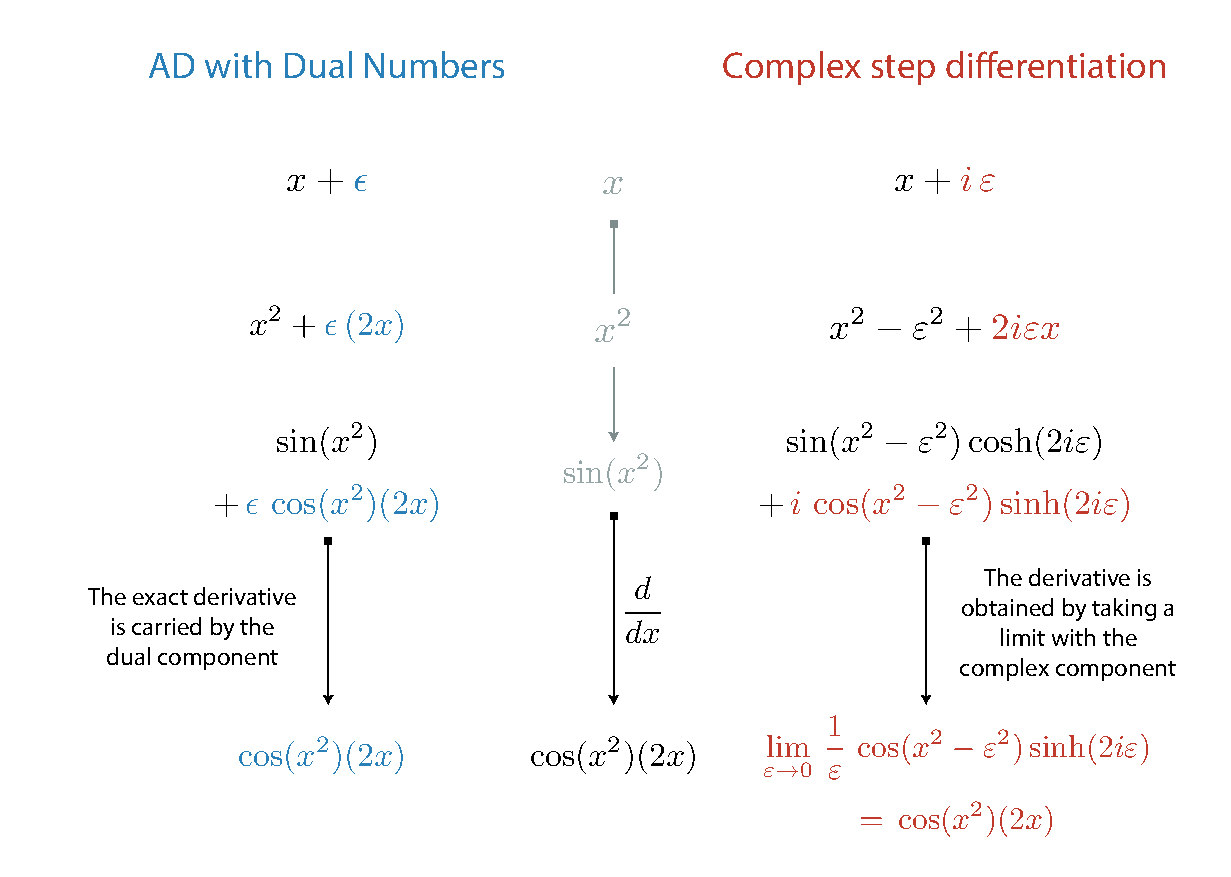
\includegraphics[width=0.75\textwidth]{tex/figures/complex-step-AD.pdf}
    \caption{Comparison between AD implemented with dual numbers and complex step differentiation. For the simple case of the function $f(x) = \sin(x^2)$, we can see how each operation is carried in the forward step by the dual component (blue) and the complex component (red). While AD gives the exact gradient at the end of the forward run, in the case of the complex step method we need to take the limit in the imaginary part. }
    \label{fig:complex-step-AD}
\end{figure}